\documentclass[11pt]{article}


\usepackage{times}
\usepackage{fancyhdr}
\usepackage{geometry}
\usepackage{graphicx}
\usepackage{amsmath}
\usepackage{cite}
\usepackage{graphicx}
\usepackage{float}
\usepackage{booktabs}
\usepackage{array}
\usepackage{hyperref}
\usepackage{titling} 
\usepackage{tocloft}
\renewcommand{\cftsecdotsep}{\cftdotsep}

% link style
\hypersetup{
    colorlinks=true,    % without outline
    urlcolor=blue,      %
    linkcolor=blue,     %
}

% paragraph
\setlength{\parindent}{0pt}
\setlength{\parskip}{12pt}
\geometry{a4paper, margin=1in}


% config page head and foot
\pagestyle{fancy}
\fancyhf{}
\fancyfoot[R]{\thepage} % L, C, R for three positions
\renewcommand{\headrulewidth}{0pt}
\setlength{\footskip}{14pt}


\title{A Weather IoT System Examination}
\author{
    Henry Wang (1576324) \and
    Yuguang Zhang (1435670) \and
    Jia zhang(1578438)
}
\date{\today}



% ========== THE START OF THIS DOCUMENT ===========
\begin{document}

% for the center first page
\begin{titlepage}
  \centering
  \vspace*{\fill}
  {\LARGE \bfseries \thetitle \par}
  \vspace{2cm}
  {\large \theauthor \par}
  \vspace{2cm}
  {\large \today \par}
  \vspace*{\fill}
\end{titlepage}

% \maketitle
\clearpage

\tableofcontents
\clearpage

% The first page flow the other pages' style
\thispagestyle{fancy}


\section{Background}

In recent years, with the development of modern human technology, the Earth's environment has been quickly changed by human activities, especially due to global climate change. Compared with the pre-industrial era, nowadays the average temperature has increased by 1.5 degrees~\cite{shaw2024automatic}. It takes more and more extreme weather and events happening in the world. It also makes weather forecasting more difficult.

The weather is affected by many factors. It is influenced by changing conditions like air temperature, air pressure, wind direction and speed, and humidity~\cite{varghese2019iot}. In common weather stations collect many different weather data, including temperature, humidity, pressure, wind speed, precipitation, light intensity, etc~\cite{shaw2024automatic}. This kind of information is always used for weather forecasting. According to Yonekura et al. 's article, they used temperature, humidity, sea level pressure, wind, precipitation intensity and rain sensors as feature vectors to train a deep neural network model to predict short-term local weather~\cite{mishra2021study}. Their deep learning model was able to successfully early 60 minutes predict precipitation intensity.


\section{Environmental Signals Collecting}

Atmospheric pressure is one of the key factors used in short-term weather forecasting. High pressure usually means calm, dry, and sunny weather, while low pressure is often linked to clouds, rain, and strong winds. Meteorologists track these pressure systems to predict how the weather will change in the coming hours or days. This helps to improve the accuracy and reliability of weather forecasts \cite{yonekura2018short} \cite{metoffice_highlow}. High and low pressure systems also affect the types of weather we experience in different seasons. In summer, high pressure often brings long periods of sunshine, heat waves, and dry conditions. In winter, it can lead to cold, dry days with frost or fog. Low pressure, on the other hand, brings unsettled weather such as storms, heavy rain, and flooding. These changes can also cause hazards like poor air quality and reduced visibility \cite{ucar_pressure}.

Temperature shows how hot or cold the air is, mainly due to heat from the sun, though human activities like greenhouse gas emissions can also affect it. Wind is caused by air moving from high-pressure areas to low-pressure areas, and the bigger the pressure difference, the stronger the wind. Humidity refers to the amount of water vapour in the air. The warmer air holds more moisture. Rain happens when water droplets in clouds become too heavy and fall to the ground \cite{metoffice_conditions} \cite{ncas_weather}.

These climate factors always influence each other. In general, if the air pressure remains at a high level, it will be a sunny day. And if the air pressure remains at a lower level. The air flows together and rises. During the rising process, it cools and forms clouds, often leading to cloudy or rainy weather \cite{mcalindon2006barometric}.


\section{Barometric Pressure Affect For Health}

McAlindon et al.'s team conducted an observational study involving 200 patients and found that barometric pressure and ambient temperature can affect knee pain in individuals with knee osteoarthritis \cite{izadyar2021effect}. They found that the number of captured seizures increased by 31.8\% when atmospheric pressure was lower than the comfortable range, and by 11.1\% when it was higher \cite{horvath2023pain}.

According to Horvath et al.'s study, there is much evidence that climate fluctuations lead to body pain for patients. This includes headaches, bone-related discomfort, neuropathic pain and others. The study also suggests that barometric pressure could be one of the contributing factors \cite{horvath2023pain}.
Changes in barometric pressure can affect blood pressure and blood sugar. Cold weather causes blood vessels to narrow, raising blood pressure. Sudden weather shifts, like storms, can also trigger similar effects, especially in older adults. For people with diabetes, low pressure can thicken blood, making it harder to control blood sugar \cite{glaser2025feel}.


\section{Architecture and Framework}

\begin{figure}[H]
    \centering
    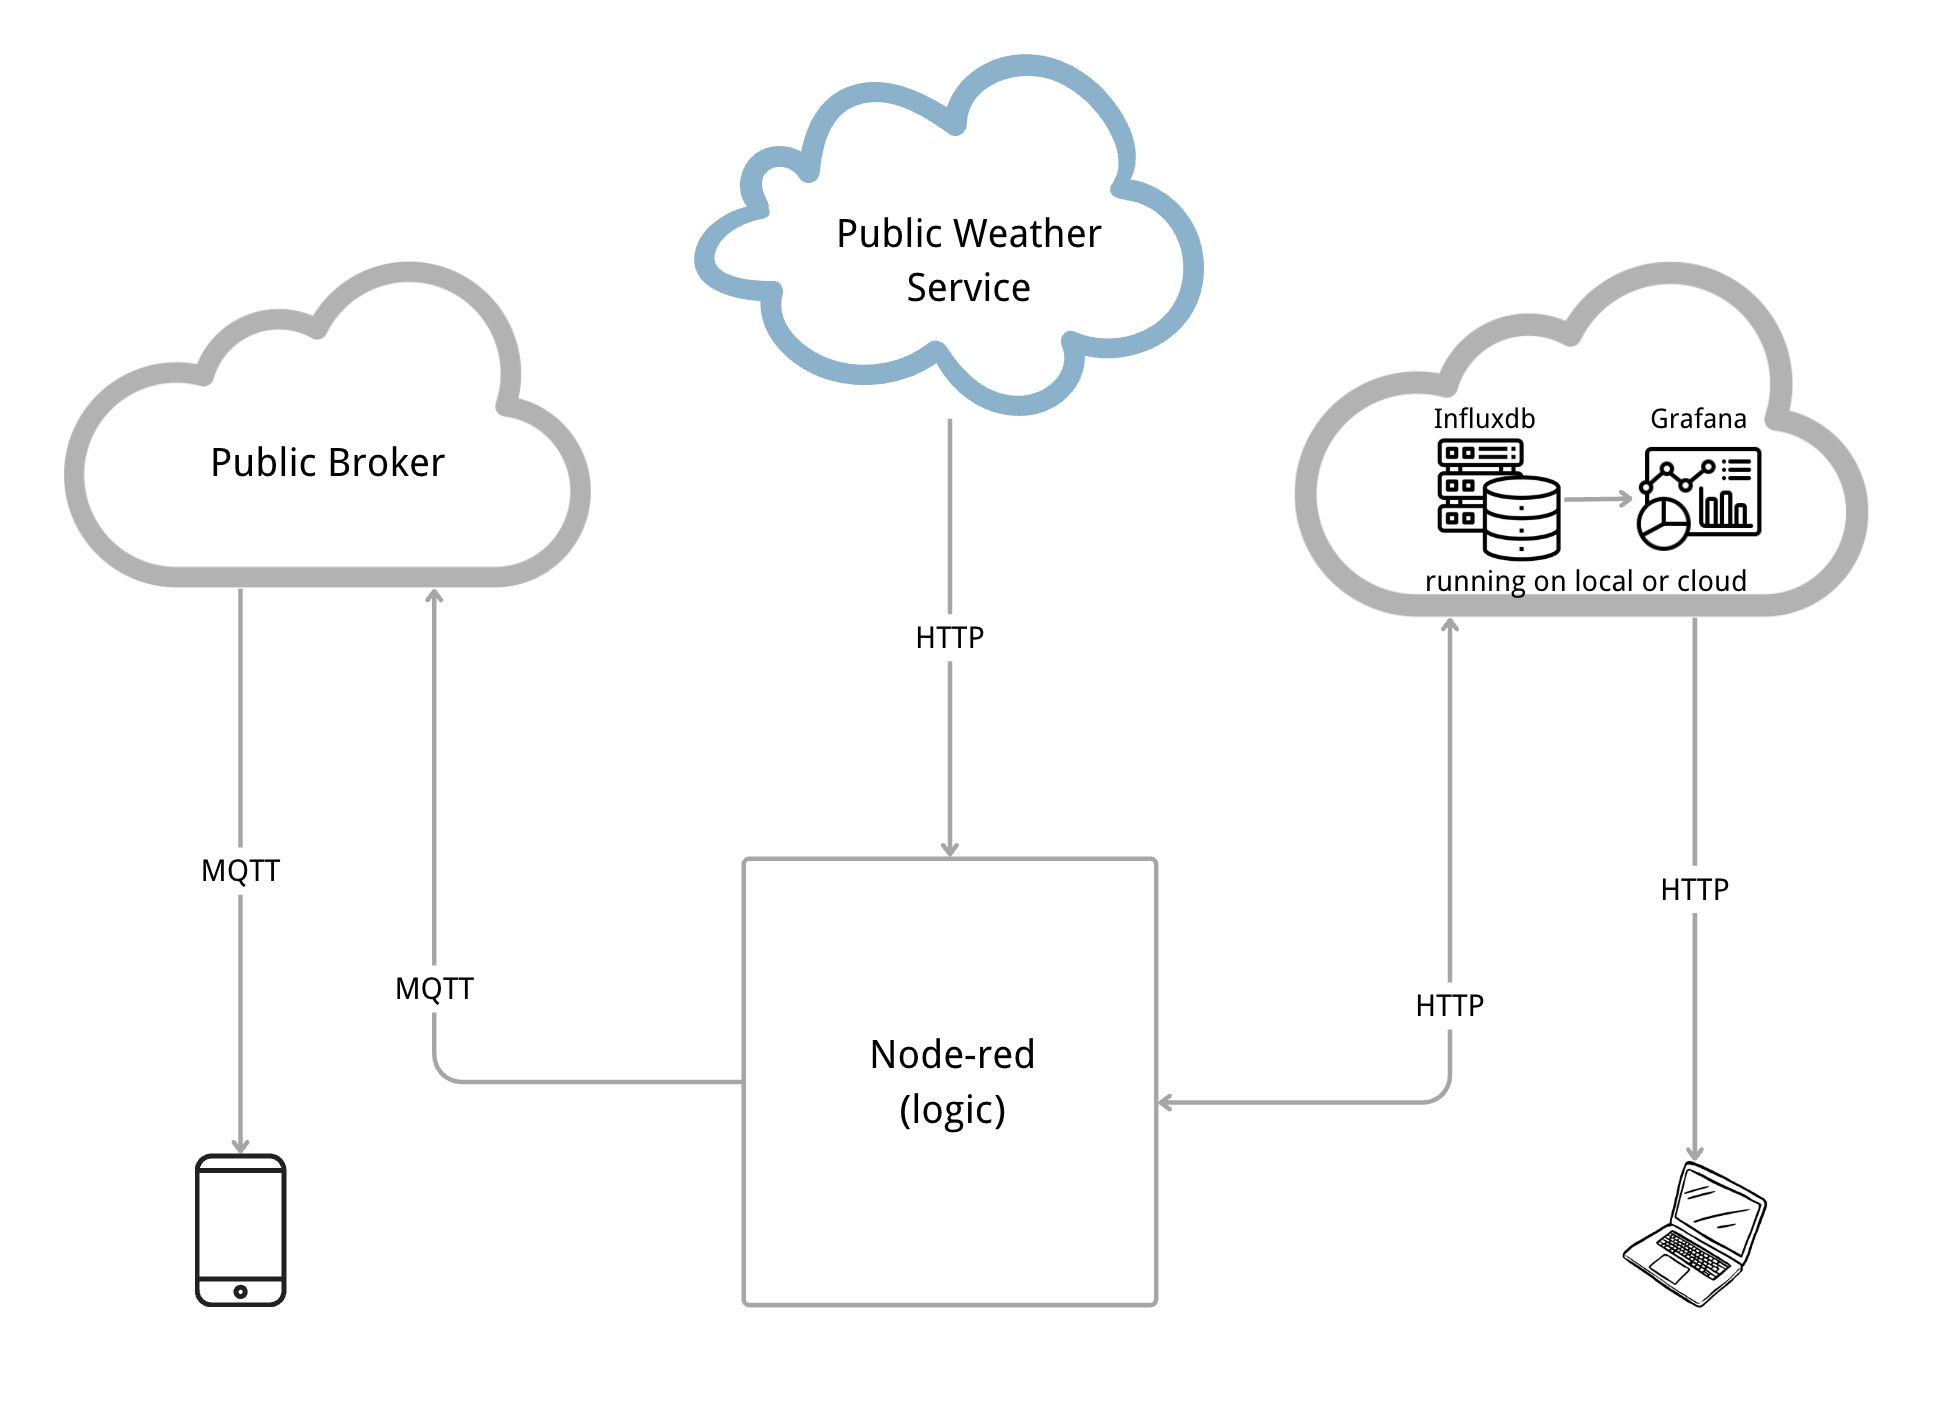
\includegraphics[width=0.8\textwidth]{pics/architecture.png}
    \caption{System architecture}
\end{figure}

\subsection{Terminal Device (Mobile Device)}
The terminal devices receive processed weather data and alarms from public broker via the MQTT protocol.

\subsection{Public Broker}
During the development phase, we use the public MQTT broker broker.emqx.io due to its simplicity and ease of access. This broker requires no installation, configuration, or authentication, making it ideal for rapid prototyping and quick testing scenarios. The broker implements two topics:

\begin{itemize}
    \item Subscribe to the topic "zzw/iot/alarm" to receive the nearest alerts for low/high temperatures and rain days forecasted over the next five days.
    \item Subscribe to "zzw/iot/weather" to receive hourly weather updates.
\end{itemize}

For production deployment, however, we plan to migrate to Mosquitto, a lightweight MQTT broker known for its enhanced security and reliability. Unlike broker.emqx.io, Mosquitto requires hosting on a server with public internet access. While this introduces additional setup requirements, it provides full control over the broker environment, allowing us to implement user authentication and enable secure TLS communication.

\subsection{Logic Center (Node-RED)}
Node-RED serves as the central logic engine of the system, orchestrating data flow and automation processes. It performs several key functions:

\begin{itemize}
    \item MQTT Publish: It communicates with the public MQTT broker to publish messages, such as alerts or weather updates.
    \item HTTP Requests: Node-RED fetches external weather data from third-party services of OpenWeather API.
    \item Data Processing: It applies automation logic—such as detecting extreme weather conditions—and generates relevant responses or alerts.
    \item Data Output: Processed data is pushed to the InfluxDB time-series database via HTTP, where it can be stored and later visualized.
    \item Data Retrieval and Forwarding: Node-RED retrieves relevant data from InfluxDB, formats it appropriately, and then publishes it back to the MQTT broker for delivery to terminal devices.
\end{itemize}

The system is designed around a decoupled data flow, meaning that data is first retrieved from the OpenWeather API and stored in the database. Only after this storage step is the data fetched again and transmitted to terminal devices. This architecture promotes cleaner, more maintainable code and ensures that each component has a clearly defined role.


\subsection{Public Weather Service}

The weather information is fetched from OpenWeather API, specifically targeting Auckland, NZ. The data includes:

\begin{itemize}
    \item Current temperature, humidity, and wind\cite{openweathermap_current_2025}
    \item Future 5-days weather forecast stepped by 3 hours\cite{openweathermap_forecast_2025}
\end{itemize}


\subsection{Data Center}
The data center component integrates three core tools to handle data storage, visualization, and communication: InfluxDB, Grafana, and Node-RED.

\subsubsection{InfluxDB (Time-Series Database)}
InfluxDB serves as the system's time-series database, storing weather data as well as system-generated alerts. It is specifically designed for time-based data such as temperature trends, humidity levels, and rainfall patterns. InfluxDB includes a built-in web UI that allows users to manage data and generate queries; however, its visualization capabilities are limited.

\subsubsection{Grafana (Visualization Layer)}
Grafana provides advanced, real-time data visualization by connecting to InfluxDB. It enables users to create dynamic dashboards and charts for monitoring weather conditions and system status at a glance. Compared to InfluxDB's native UI, Grafana offers a wider variety of chart types and supports integration with multiple data sources, making it suitable for complex dashboards.

Both InfluxDB and Grafana are available as multi-platform tools, allowing installation on various operating systems. Additionally, users and developers can choose to access their public hosted services to avoid local installation.

\subsubsection{Node-RED (Data Flow and Integration)}
Node-RED is used to manage the flow of data into and out of InfluxDB. It pushes weather and alert data into the database and can retrieve historical or forecasted information for further processing or for redistribution via MQTT. The Node-RED plugin used for InfluxDB integration is available at: node-red-contrib-influxdb\cite{nodered_influxdb_2025}.

\subsubsection{Deployment Strategy}
During development, InfluxDB and Grafana are deployed locally using Docker containers, which simplifies setup and testing. For production, both services will be migrated to a virtual private server (e.g., AWS), ensuring stable internet connectivity, improved performance, and higher reliability.


\section{Communication protocols}

\begin{itemize}
    \item MQTT: Lightweight, ideal for pushing frequent updates like hourly weather or alarms.
    \item HTTP: Used for retrieving third-party data and pushing it to the database.
\end{itemize}

Security Considerations:
\begin{itemize}
    \item broker.emqx.io: Offers basic encryption (TLS) but may expose data to the public.
    \item Mosquitto (self-hosted): Allows for complete control over encryption and access. TLS and authentication can be enforced, improving security.
    \item Node-RED: While capable of secure HTTP and MQTT with TLS, the level of security depends on the environment setup.
\end{itemize}




\section{Workflow Summary}

\begin{enumerate}
    \item Node-RED fetches weather data from OpenWeather.
    \item Weather data is stored in InfluxDB.
    \item Grafana reads from InfluxDB to provide real-time dashboards.
    \item Node-RED fetch data from InfluxDB.
    \item Node-RED forward information to the public broker.
    \item Public broker publishes alerts and weather updates to mobile devices.
\end{enumerate}

\begin{figure}[H]
    \centering
    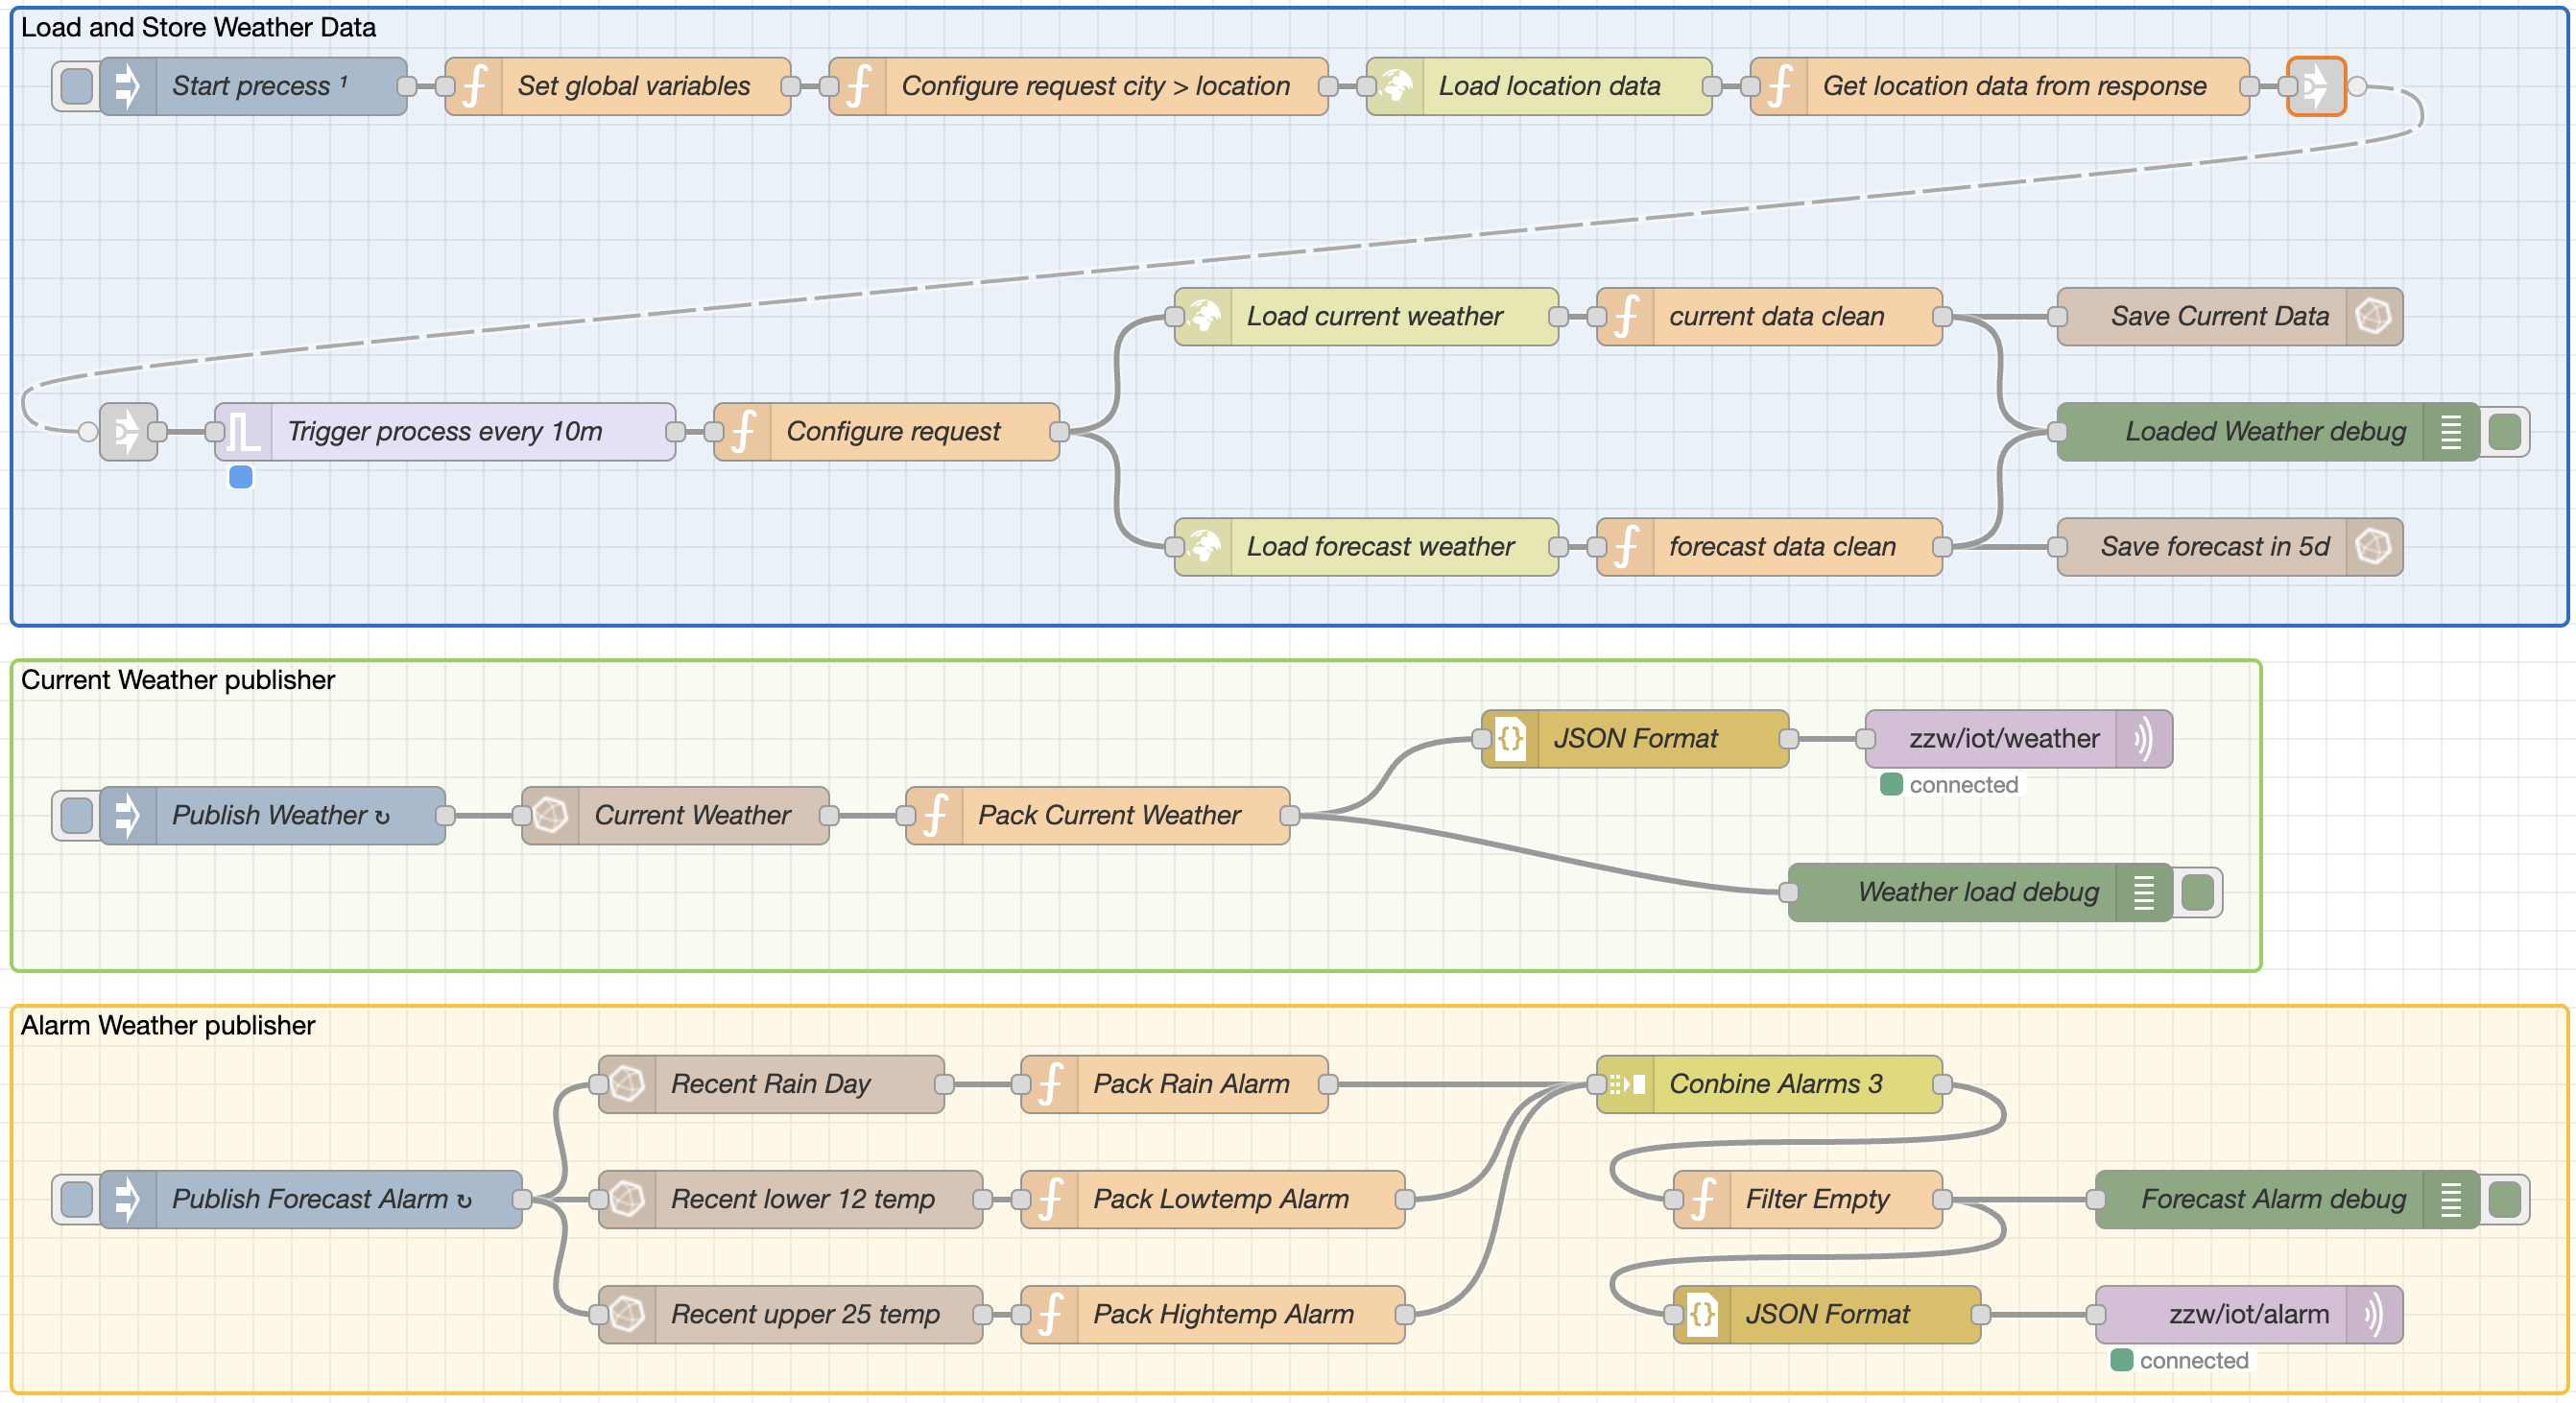
\includegraphics[width=\textwidth]{pics/workflow.png}
    \caption{The workflow of logic center}
\end{figure}


\section{Test Plan}

\subsection{Objectives}
\begin{itemize}
    \item Ensure accurate weather data retrieval and alert generation.
    \item Validate reliable data flow across APIs, MQTT topics, and the database.
\end{itemize}

\subsection{Scopes}
\begin{itemize}
    \item Node-RED logic for HTTP fetch, alert logic, and MQTT publishing.
    \item OpenWeather API interaction.
    \item MQTT communication (zzw/iot/alarm, zzw/iot/weather).
    \item InfluxDB write operations.
\end{itemize}

\subsection{Test Types}
\begin{itemize}
    \item Weather Data Fetching: Node-RED fetches from OpenWeather at scheduled intervals via HTTP.
    \item InfluxDB Integration: Data is correctly written to InfluxDB with valid timestamps and fields.
    \item Alert Generation: High/low temperature or rain day triggers correctly detect conditions from forecast data.
    \item Weather Data Publishing: Current and forecast weather data is processed and published to zzw/iot/weather.
    \item End-to-End Data Flow: Verify full pipeline: API → Node-RED → MQTT/InfluxDB; Confirm output matches input (e.g. temperature values and timestamps).
\end{itemize}

\subsection{Entry Criteria}
\begin{itemize}
    \item Node-RED flows deployed.
    \item OpenWeather API key configured.
    \item OpenWeather API key configured.
    \item InfluxDB instance running.
\end{itemize}

\subsection{Exit Criteria}
\begin{itemize}
    \item All functional and API paths tested.
    \item System demonstrates stable data flow and correct alert behavior.
\end{itemize}




\subsection{Test Cases (5)}
\renewcommand{\arraystretch}{1.5}
\begin{table}[ht]
\centering
\begin{tabular}{|>{\raggedright\arraybackslash}p{4cm}|p{10cm}|}
\hline
\textbf{ID} & TC-1 \\
\hline
\textbf{Title} & Verify that Node-RED fetches weather data via HTTP from OpenWeather APIs \\
\hline
\textbf{Preconditions} & Node-RED is deployed and configured with the correct API key \\
\hline
\textbf{Steps} & \vspace{-20pt}
\begin{enumerate}
    \item Deploy Node-RED flow with HTTP request node
    \item Trigger data fetch
    \item Observe debug node or log
\end{enumerate} \\
\hline
\textbf{Expected Result} &  \vspace{-20pt}
\begin{enumerate}
    \item Node-RED successfully fetched current weather data and 5-day forecast using HTTP.
    \item JSON structure matched expectations.
\end{enumerate} \\
\hline
\textbf{Actual Result} &  \vspace{-20pt}
\begin{enumerate}
    \item Node-RED successfully fetched current weather data and 5-day forecast using HTTP.
    \item JSON structure matched expectations.
\end{enumerate} \\
\hline
\textbf{Case Status} & Passed \\
\hline
\end{tabular}
\caption{Test Case TC-1}
\label{tab:tc1}
\end{table}
\begin{table}[ht]
\centering
\begin{tabular}{|>{\raggedright\arraybackslash}p{4cm}|p{10cm}|}
\hline
\textbf{ID} & TC-02 \\
\hline
\textbf{Title} & Verify that weather data is correctly written to InfluxDB \\
\hline
\textbf{Preconditions} & InfluxDB is running and accessible \\
\hline
\textbf{Steps} & \vspace{-20pt}
\begin{enumerate}
    \item Allow Node-RED to send parsed data to InfluxDB
    \item Use InfluxDB CLI or UI to query recent data
\end{enumerate} \\
\hline
\textbf{Expected Result} & Data points appeared in InfluxDB with correct timestamps. \\
\hline
\textbf{Actual Result} & Data points appeared in InfluxDB with correct timestamps. \\
\hline
\textbf{Case Status} & Passed \\
\hline
\end{tabular}
\caption{Test Case TC-02}
\label{tab:tc2}
\end{table}
\begin{table}[ht]
\centering
\begin{tabular}{|>{\raggedright\arraybackslash}p{4cm}|p{10cm}|}
\hline
\textbf{ID} & TC-03 \\
\hline
\textbf{Title} & Verify that Node-RED triggers high/low temperature alerts \\
\hline
\textbf{Preconditions} & Valid 5-day forecast data fetched \\
\hline
\textbf{Steps} & \vspace{-20pt}\begin{enumerate}
    \item Inject mock forecast data with temperature > threshold
    \item Observe flow logic execution
    \item Check MQTT publish to topic zzzw/iot/alarm
\end{enumerate} \\
\hline
\textbf{Expected Result} & Node-RED triggered a high-temperature alert and published a correctly formatted MQTT message to zzzw/iot/alarm \\
\hline
\textbf{Actual Result} & Node-RED triggered a high-temperature alert and published a correctly formatted MQTT message to zzzw/iot/alarm \\
\hline
\textbf{Case Status} & Passed \\
\hline
\end{tabular}
\caption{Test Case TC-03}
\label{tab:tc3}
\end{table}
\begin{table}[ht]
\centering
\begin{tabular}{|>{\raggedright\arraybackslash}p{4cm}|p{10cm}|}
\hline
\textbf{ID} & TC-04 \\
\hline
\textbf{Title} & Verify that current and forecast weather data is published to MQTT topic zzzw/iot/weather \\
\hline
\textbf{Preconditions} & Weather data has been written correctly into InfluxDB \\
\hline
\textbf{Steps} & \vspace{-20pt}\begin{enumerate}
    \item Parse and format the result
    \item Send message to MQTT broker
\end{enumerate} \\
\hline
\textbf{Expected Result} & MQTT messages were sent at regular intervals containing JSON formatted weather data \\
\hline
\textbf{Actual Result} & MQTT messages were sent at regular intervals containing JSON formatted weather data \\
\hline
\textbf{Case Status} & Passed \\
\hline
\end{tabular}
\caption{Test Case TC-04}
\label{tab:tc4}
\end{table}
\begin{table}[ht]
\centering
\begin{tabular}{|>{\raggedright\arraybackslash}p{4cm}|p{10cm}|}
\hline
\textbf{ID} & TC-05 \\
\hline
\textbf{Title} & Verify full workflow: API $\rightarrow$ Node-RED $\rightarrow$ InfluxDB/MQTT \\
\hline
\textbf{Preconditions} & ALL services are online \\
\hline
\textbf{Steps} & \vspace{-20pt}\begin{enumerate}
    \item Fetch weather data from OpenWeather
    \item Observe alert logic and publishing
    \item Confirm MQTT and InfluxDB both receive valid output
\end{enumerate} \\
\hline
\textbf{Expected Result} & \vspace{-20pt}\begin{enumerate}
    \item Input from OpenWeather matched values seen in both MQTT output and InfluxDB records
    \item No data loss or mismatch detected.
\end{enumerate} \\
\hline
\textbf{Actual Result} & \vspace{-20pt}\begin{enumerate}
    \item Input from OpenWeather matched values seen in both MQTT output and InfluxDB records
    \item No data loss or mismatch detected
\end{enumerate} \\
\hline
\textbf{Case Status} & Passed \\
\hline
\end{tabular}
\caption{Test Case TC-05}
\label{tab:tc5}
\end{table}
\clearpage

\bibliographystyle{IEEEtran}
% ref.bib
\bibliography{ref}



\end{document}
